%!TEX root = ../../../report.tex
\section{Joints} % (fold)
\label{sec:joints}
Following the idea of mimicking the human lower-body structure it was decided to implement three actuated rotational joints per leg although some research was conducted on the use of passive ankles as in \cite{dacbot1}, \cite{phides} or \cite{mabel}.
However, the results introduced in \cite{grimmer} from their analysis of joint actuation for prosthetics limbs proved the importance of the actuation in the ankles for running.

The design of the joints entailed the addressing of three main areas

\begin{itemize}
  \item Actuator model
  \item Transmission system
  \item Implementation of dedicated compliance
\end{itemize}

% \begin{figure}[ht!]
%   \centering
%   \includegraphics[width=\textwidth]{figures/20160518_195014.jpg}
%   \caption{Might help}
%   \label{fig:figure1}
% \end{figure}

\subsection{Actuators} % (fold)
\label{sub:actuators}
In humans, the actuation of the joints is mostly provided by pairs of agonist-antagonist skeletal muscles linked to the bones through the tendons \cite{anatomy}.
The activation-inhibition of these muscles produce a lever effect on the bones that leads to its control and motion by modifying the angle between two consecutive limbs.
To achieve the same kind of motion control, the implementation of a similar system through electric linear actuators was considered.
However, the time constraints, their price and their complexity led to discard them and select conventional electric motors.
The selected motor model will have to be able to provide a sufficient torque to generate the desired forces at the end of the link, following equation \ref{eq:torque}.

\begin{equation}
\label{eq:torque}
  \tau = r \times F
\end{equation}

This equation could be sufficient to compute the torque required by the load for a motor application of leverage. 
However, an study of each joint separately would not provide an accurate enough solution due to the configuration of the legs, making necessary an study of the actuation as for a kinematic chain.
The analysis of the actuators requirements is to be found in \ref{cha:mathematical_model}.

% subsection actuators (end)

\subsection{Transmission} % (fold)
\label{sub:transmission}
As introduced in \ref{sub:moments_of_inertia}, the reduction of the moments of inertia in the limbs in order to minimize the torque requirements for motion was set as a priority.
This led to the study of methods to displace the CoM of the limbs as close to their joints axes as possible, thus reducing their inertias.
The solution was to place the actuators, the heaviest components of the design, as close to the upper part of the frame as possible, which would also result in the allocation of the CoM of the frame upper in the sagital plane.
An schematic example of this idea can be seen in the Figures in \ref{fig:compliance} for the ankle actuation, where the motor has been placed under the knee axis. 
The same principle has been applied to the knee actuation, as can be seen in the final implementation. 
For the hip, however, it was not necessary to install a transmission system, but a gear mechanism whose justification is to be found in \ref{cha:mathematical_model}.

Due to the new arrangement, a powertrain was required to transmit the torque to the joints.
It was decided to implement a system of 2 pulleys + belt due to its simplicity and optimal capabilities for the project requirements.
The goal of this mechanism is only the transmission of power, without any further adjustment of angular speed-torque ratios.
The calculations to find the optimal dimensions of the system are contained in \ref{sub:pulleys_and_belts}.
The pitfall of this implementation, however, is the introduction of delays in the motion transmission and the natural loss of accuracy arisen from the backlash associated to the use of pulleys.
Modeling these uncertainties for a classic locomotion controller based on the motion equations is proved a complex task. 
However it was assumed here that the ANN controllers that would drive the RuBi platform would be able to adapt to them without a model of the robot.

%Reduction of the moments of inertia
%Introduction of delays and loss of accuracy 

% subsection transmission (end)

\subsection{Compliance} % (fold)
\label{sub:compliance}

%Flexible vs stiff drive train
%Power peak and average consumption comparisons --> energy storage 
%Protection against impact forces on landing phase


\begin{figure}[hb!]
\label{fig:compliance}
  \begin{subfigure}{.19\textwidth}
    \centering
    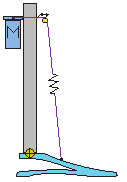
\includegraphics[width=\linewidth]{figures/illustration_serial_pulley.pdf}
    \caption{Serial pulley}
    \label{fig:series_pulley}
  \end{subfigure}
  \begin{subfigure}{.19\textwidth}
    \centering
    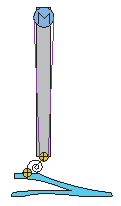
\includegraphics[width=\linewidth]{figures/illustration_serial_rotational.pdf}
    \caption{Series rotational}
    \label{fig:series_rotational}
  \end{subfigure}
  \begin{subfigure}{.19\textwidth}
    \centering
    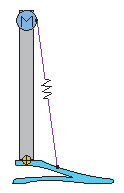
\includegraphics[width=\linewidth]{figures/illustration_serial_direct_i.pdf}
    \caption{Series direct 1}
    \label{fig:series_direct_i}
  \end{subfigure}
  \begin{subfigure}{.19\textwidth}
    \centering
    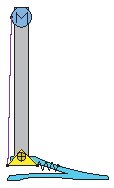
\includegraphics[width=\linewidth]{figures/illustration_serial_direct_ii.pdf}
    \caption{Series direct 2}
    \label{fig:series_direct_ii}
  \end{subfigure}
  \begin{subfigure}{.19\textwidth}
    \centering
    \includegraphics[width=\linewidth]{figures/illustration_serial_elastic_band.pdf}
    \caption{Series elastic band}
    \label{fig:series_elastic_band}
  \end{subfigure}
\end{figure}  

% subsection compliance (end)

% section joints (end)